% !TeX root = autocomplete.tex
\documentclass[a4paper]{article}
\usepackage{todonotes}
\usepackage[colorlinks, urlcolor=blue, linkcolor=blue]{hyperref}
\usepackage{multicol}
\usetikzlibrary{shapes,arrows}
\usepackage{dirtree}


\newcommand{\cursor}{%
\begin{tikzpicture}[remember picture, overlay]%
%    \begin{scope}[transparency group]
		\draw[color=blue, very thick, opacity=0.3] (0, 0.3) -- (0, -0.08);
		\draw[color=blue, very thick, opacity=0.3] (-0.1, -0.1) -- (0.1, -0.1);
%    \end{scope}
\end{tikzpicture}%
}

\newcommand{\selection}[1]{%
\begin{tikzpicture}[remember picture, overlay]%
\node [coordinate] (selectionStart) {};%
\end{tikzpicture}%
#1%
\begin{tikzpicture}[remember picture, overlay]%
\fill[color=blue, opacity=0.3] (selectionStart)++(0, -0.1) rectangle (0, 0.3);
\end{tikzpicture}%
}


\title{Documentation for TeXworks autocompleter}
\author{Henrik Skov Midtiby}

\begin{document}
\maketitle

\begin{abstract}
TeXworks is a powerfull latex editor which can be extended 
through scripts written in javascript.
This script is an attempt at adding autocompletion capability 
to the TeXworks editor.
Currently it can complete references, citations, filenames,
words present in the open files and items in a list of templates.
\end{abstract}

\section{What the script can do?}
\label{secWhatCanTheScriptDo}

The script can do context based completions in latex documents.
By looking at open files (*.tex and *.bib) and contents of the 
local directory, the script can complete
\begin{itemize}
\item	references, defined with label in open files
\item	citations, used in opened files and in open bibtex files
\item	filenames, based on directory content
\end{itemize}

All interaction with the script consists of activating it using 
its shortcut \mbox{crtl + m}. 
In a document with the content shown in figure 
\ref{figExampleDocument}, the script will generate the following 
completions.
In the first line, the cursor location is marked with\cursor, 
in the following lines the selected text is marked as \selection{this}.
%
\begin{multicols}{3}
\noindent
hiera\cursor	\\
hierarchy\cursor

\columnbreak
\noindent
h\cursor	\\
hi\selection{erarchy} \\
hi\selection{eroglyphs} \\

\columnbreak
\noindent
\textbackslash ref\{h\cursor	\\
\textbackslash ref\{he\selection{lloWorld} \\
\textbackslash ref\{he\selection{rons} \\
\textbackslash ref\{he\selection{lloWorld}
\end{multicols}

If there is a single completion candidate, the candidate is inserted 
and you can continue writing.
If multiple candidates exists, the first candidate is inserted with 
the last part of it selected; when the script is activated again the 
next completion candidate is inserted, this is continued until all 
candidates have been shown and the first is inserted again.



\begin{figure}[t]
\centering
\begin{verbatim}
\section{Hello world}
\label{helloWorld}

Some text about hierarchy and hieroglyphs.

\begin{align}
\label{herons}
A
	& = \sqrt{s \cdot (s - a) \cdot (s - b) \cdot (s - c)}
\end{align}
\end{verbatim}
\caption{Example document containing references and labels used in section \ref{secWhatCanTheScriptDo}.}
\label{figExampleDocument}
\end{figure}

\subsection{See the script in action}
\label{ssecSeeTheScriptInAction}

The following two videos demonstrates how the script can be used.
%
\begin{itemize}
\item	Demonstration of context aware autocompletion for texworks\\
		\url{http://www.youtube.com/watch?v=wTjyiik9xm0}
\item	Autocompleter for TeXworks\\
		\url{http://www.youtube.com/watch?v=gRSq_OSxPec}
\end{itemize}


\subsection{How to install the script}
\label{ssecHowToInstallTheScript}

Download \texttt{autocomplete.js} and 
\texttt{autocompleteFunctions.js}\footnote{\url{https://github.com/henrikmidtiby/TeXworks-scripts/tree/master/autocomplete}} and place them in a subfolder of your 
TeXWorks scripts dir.




\section{How does it work}
\label{secHowDoesItWork}

\subsection{State representation}

The script relies on a state representation that contains information 
about what should be completed and the last suggestion presented to 
the user.
What should be completed is in front of the cursor and the last 
suggestion is stored in the selected area.
As an example take the following string

eqnP\selection{Testing}	\\
\noindent
The representation is given as two parts \emph{eqnP} and \emph{Testing}.
The last suggestion is found by combining the two parts of the 
representation, which gives \emph{eqnPTesting}.
From the first part (\emph{eqnP}) can the list of completion candidates 
be determined and with the last part (\emph{Testing}) it is possible to 
determine the next element to suggest.




\subsection{Context recognition}

\begin{figure}
\centering
% !TeX root = ../autocomplete.tex
% Define block styles
\tikzstyle{decision} = [rectangle, draw, fill=green!20, 
    text width=9em, text centered, rounded corners, minimum height=2em]
\tikzstyle{block} = [rectangle, draw, fill=blue!20, 
    text width=9em, text centered, rounded corners, minimum height=2em]
\tikzstyle{line} = [draw, -latex']

\begin{tikzpicture}[node distance=1.5cm, auto]
	% Draw nodes
	% Activate script
	\node [block] (activate) {activate script};
	% First in line, -> close environment
	\node [decision, below of=activate] (firstInInlineQ) {Cursor placed first in line?};
	\node [block, right of=firstInInlineQ, node distance=5cm] (closeEnvironment) {Close environment};
	% Suggest command or environment
	\node [decision, below of=firstInInlineQ] (suggestCommand) {Can command be completed?};
	\node [block, right of=suggestCommand, node distance=5cm] (insertCommand) {Suggest command};
	% addLabelBelow
	\node [decision, below of=suggestCommand] (addLabelBelowQ) {At end of section or similar?};
	\node [block, right of=addLabelBelowQ, node distance=5cm] (suggestLabel) {Suggest label};
	% should complete filename
	\node [decision, below of=addLabelBelowQ] (completeFilenameQ) {Can a filename be completed?};
	\node [block, right of=completeFilenameQ, node distance=5cm] (completeFilename) {Suggest filename};
	% should complete argument to macro
	\node [decision, below of=completeFilenameQ] (completeArgumentToMacroQ) {Can complete ref, label or citation?};
	\node [block, right of=completeArgumentToMacroQ, node distance=5cm] (completeArgumentToMacro) {Suggest completion};
	% complete based on words in file
	\node [block, below of=completeArgumentToMacroQ] (wordCompletion) {Suggest word};

	% Stop
	\node [block, below of=activate, node distance=10.5cm, xshift=8cm] (stop) {stop};

	% Draw edges
	% Activate script
	% First in line, -> close environment
	\path [line] (activate) -- (firstInInlineQ);
	\path [line] (firstInInlineQ) -- node {yes} (closeEnvironment);
	\path [line] (closeEnvironment) -| (stop);
	% Suggest command or environment
	\path [line] (firstInInlineQ) -- node {no} (suggestCommand);
	\path [line] (suggestCommand) -- node {yes} (insertCommand);
	\path [line] (insertCommand) -| (stop);
	% addLabelBelow
	\path [line] (suggestCommand) -- node {no} (addLabelBelowQ);
	\path [line] (addLabelBelowQ) -- node {yes} (suggestLabel);
	\path [line] (suggestLabel) -| (stop);
	% should complete filename
	\path [line] (addLabelBelowQ) -- node {no} (completeFilenameQ);
	\path [line] (completeFilenameQ) -- node {yes} (completeFilename);
	\path [line] (completeFilename) -| (stop);
	% should complete argument to macro
	\path [line] (completeFilenameQ) -- node {no} (completeArgumentToMacroQ);
	\path [line] (completeArgumentToMacroQ) -- node {yes} (completeArgumentToMacro);
	\path [line] (completeArgumentToMacro) -| (stop);
	% complete based on words in file
	\path [line] (completeArgumentToMacroQ) -- node {no} (wordCompletion);
	\path [line] (wordCompletion) -| (stop);


\end{tikzpicture}

\caption{Flow chart.}
\label{figFlowChart}
\end{figure}


\subsubsection{Close environment}
\label{sssecCloseEnvironment}

Open environments can be closed by placing the cursor first
in the line where the environment should be closed.
The script can handle nested environments by only closing
previously unclosed environments.

\begin{multicols}{2}
\noindent
Before \\
\textbackslash begin\{center\}\\
\cursor

\columnbreak
\noindent
After \\
\textbackslash begin\{center\}\\
\textbackslash end\{center\}\\
\cursor
\end{multicols}


\begin{multicols}{2}
\noindent
Before \\
\textbackslash begin\{center\}\\
\textbackslash begin\{itemize\}\\
\textbackslash item\\
\cursor

\columnbreak
\noindent
After \\
\textbackslash begin\{center\}\\
\textbackslash begin\{itemize\}\\
\textbackslash item\\
\textbackslash end\{itemize\} \\
\textbackslash end\{center\} \\
\cursor
\end{multicols}


\subsubsection{Suggest command or template}
\label{sssecSuggestCommandOrTemplate}

\noindent
\textbackslash include\cursor \\
\textbackslash include\selection{graphics}\\
\textbackslash include\selection{only}\\
\textbackslash include\selection{graphics\{filename\}}



\subsubsection{Suggest label}
\label{sssecSuggestLabel}

Place the cursor at the end of a line containing a section, subsection 
or similar, activate the script and a label for the section / subsection
will be suggested.



\begin{multicols}{2}
\noindent
Before \\
\textbackslash subsubsection\{Suggest label\}\cursor\\

\columnbreak
\noindent
After \\
\textbackslash subsubsection\{Suggest label\}\\
\textbackslash label\{sssecSuggestLabel\}\cursor
\end{multicols}

\noindent
It also works inside figure and table environments after the 
caption command as shown below.
%
\begin{multicols}{2}
\noindent
Before \\
\textbackslash begin\{figure\}		\\
\textbackslash centering		\\
\textbackslash includegraphics[width=6cm]\{\}		\\
\textbackslash caption\{Testing\}\cursor		\\
\textbackslash end\{figure\}

\columnbreak
\noindent
After \\
\textbackslash begin\{figure\}		\\
\textbackslash centering		\\
\textbackslash includegraphics[width=6cm]\{\}		\\
\textbackslash caption\{Testing\}		\\
\textbackslash label\{figTesting\}\cursor		\\
\textbackslash end\{figure\}
\end{multicols}







\subsubsection{Suggest filename}
\label{sssecSuggestFilename}

Arguments to macros like include, input and includegraphics that 
accept filenames can be completed based on the files in the current 
directory structure.
The following completion sequences can be observed in a directory 
structure as shown in figure \ref{figDirectoryStructure}.

\begin{multicols}{2}
\noindent
\textbackslash include\{\cursor \\
\textbackslash include\{\selection{autocomplete.aux} \\
\textbackslash include\{\selection{autocomplete.tex}


\columnbreak
\noindent
\textbackslash includegraphics\{pic\slash \cursor \\
\textbackslash includegraphics\{pic\slash flowdiagram.tikz\cursor

\end{multicols}

\begin{figure}[h]
\dirtree{%
.1 Current directory.
.2 autocomplete.aux.
.2 autocomplete.tex.
.2 pic.
.3 flowdiagram.tikz.
}
\caption{Example directory structure used in section 
\ref{sssecSuggestFilename}.}
\label{figDirectoryStructure}
\end{figure}



\subsubsection{Suggest ref, label or citation}
\label{sssecSuggestRefLabelOrCitation}

References completed based on observed arguments to macros like
label, ref, pageref and eqref in all files currently opened by 
TeXworks.
A similar approach is used for completing arguments to label and 
cite commands.
When completing cite commands the script also searches for candidates 
in open bibtex files.

\begin{multicols}{2}
\noindent
\textbackslash ref\{eq\cursor \\
\textbackslash ref\{eq\selection{nMaxHeight} \\
\textbackslash ref\{eq\selection{nSurf} \\
\textbackslash ref\{eq\selection{nVol} 


\columnbreak
\noindent
\phantom{d}
\end{multicols}


\subsubsection{Suggest word}
\label{sssecSuggestWord}
    
\begin{multicols}{3}
\noindent

\columnbreak
\noindent

\columnbreak
\noindent
\end{multicols}


\subsection{Insert common text present in all candidates}

\section{Feedback and suggestions}

If you have any feedback or suggestions about the script, feel 
free to contact me on \texttt{henrikmidtiby@gmail.com}.

\end{document}